% !TEX TS-program = pdflatex
% !TEX encoding = UTF-8 Unicode

% !TEX root = vortrag.tex
% !TEX encoding = UTF-8 Unicode

\documentclass[t, ngerman]{beamer} %compress,

%% Pakete laden...
  \usepackage[T1]{fontenc}
  \usepackage[utf8]{inputenc}
  \usepackage{
      babel,
      bookmark,
      booktabs,
%      blindtext,
      colortbl,
%      eurosym,
      graphicx,
	  hyperref,
%      libertine,
      microtype,
      pifont,
      pgfpages,
      tikz,
%      xspace,
  }


%% Design festlegen...
  \mode<presentation>{
%      \useoutertheme[subsection=false]{smoothbars}
      \useinnertheme{rectangles} % rectangles, circles, rounded
      \usecolortheme[RGB={153,0,0}]{structure}
      \definecolor{unihd}{RGB}{153,0,0}
      \definecolor{dark}{RGB}{115,0,0}
      \definecolor{light}{RGB}{241,229,229}
      \usecolortheme{whale}
		 \usecolortheme{orchid}
%	   \usecolortheme{beaver}
%      \setbeamercovered{transparent}
      \beamertemplatenavigationsymbolsempty
%      \setbeameroption{show notes on second screen}
      \setbeamertemplate{note page}[plain]
      \logo{
\includegraphics[width=3.5cm]{fs-logo-small}}

  }

%% nützliche Definitionen...
  \graphicspath{{media/}}

%% Titelinformationen...
  \title[Studienverwaltung$\mu$]{Das Müsli und das LSF\\\small oder: wer wie was wo Stundenplan}
  \author[
	koebi
  ]{
	Jakob Schnell\\{\scriptsize\url{koebi@mathphys.stura.uni-heidelberg.de}}
  }
%  \institute{  
\includegraphics[width=5.5cm]{fs-logo-big} }

  \date{\vspace*{-2em}\\ 01. Oktober 2018}

  \hypersetup{
      pdfauthor={Jakob Schnell},
      pdftitle={Müsli-Vortrag},
      pdfsubject={hihi},
      pdfkeywords={1},
      pdfpagelayout={SinglePage},
  }
  


\newenvironment{rcases}{%
  \left.\renewcommand*\lbrace.%
  \begin{cases}}%
{\end{cases}\right\rbrace}


\begin{document}
\begin{frame}[plain]
	   \bookmark[level=0, page=1]{Titel}
	   \titlepage
  		\tikz[,overlay]
     \node at
        (current page.south)
		{
\includegraphics[width=6cm]{fs-logo_4c}};
\end{frame}

\iffalse
\begin{frame}{Übersicht}
  \bookmark[level=0, page=2]{Inhalt}
  \tableofcontents
    \note{\tableofcontents}
\end{frame}
\fi

\section{Einführung}
\begin{frame}{Systeme der Universität}
    \begin{itemize}
        \only<1>{
            \item \textbf{M}athematisches \textbf{Ü}bungsgruppen und \textbf{S}chein\textbf{l}isten\textbf{i}nterface
        }
        \visible<2->{
           \item \textbf{Müsli}
        }
        \visible<4->{
            \begin{itemize}
                \item Übungsgruppenverwaltung in der Mathe
                \item einfach, intutitiv und toll
                \item einzig gutes System in Heidelberg
            \end{itemize}
        }
        \vfill
        \only<2>{
            \item \textbf{L}ehre, \textbf{S}tudium und \textbf{F}orschung
        }
        \visible<3->{
            \item \textbf{LSF}
        }
        \visible<5->{
                \begin{itemize}
                \item Vorlesungsverzeichnis
                \item Studiums/Prüfungsverwaltung
                \item theoretisch Raumverwaltung
            \end{itemize}
        }
        \vfill
        \visible<3->{
           \item \textbf{Moodle}
        }
        \visible<6->{
            \begin{itemize}
                \item E-Learning-Plattform
                \item viel benutzt in der Info
            \end{itemize}
        }
        \visible<7->{
           \item \textbf{MaMpf}
        }
        \vfill
    \end{itemize}
\end{frame}

\section{Das Moodle}
\begin{frame}{Das moodle}
    \vspace*{10pt}
    \makebox[\linewidth]{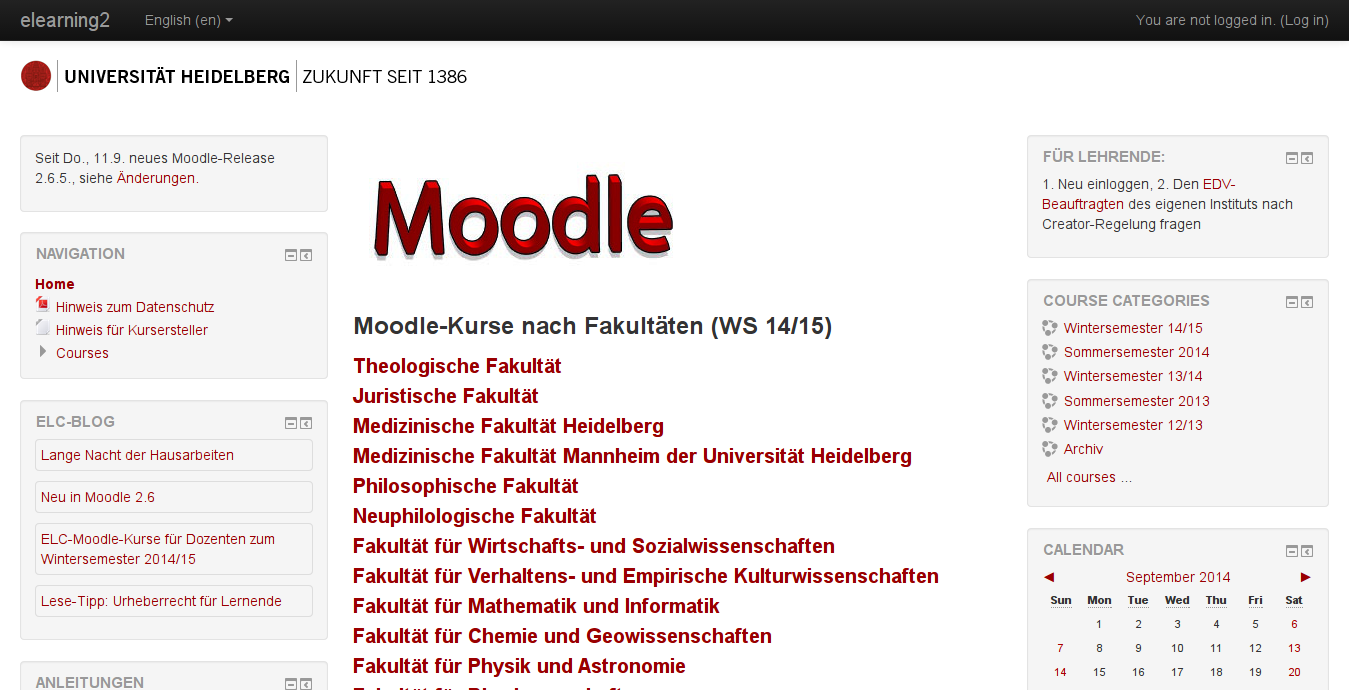
\includegraphics[width=\paperwidth]{moodle_start_2014.png}}
\end{frame}

\begin{frame}{Anmeldung}
    \vspace*{10pt}
    \makebox[\linewidth]{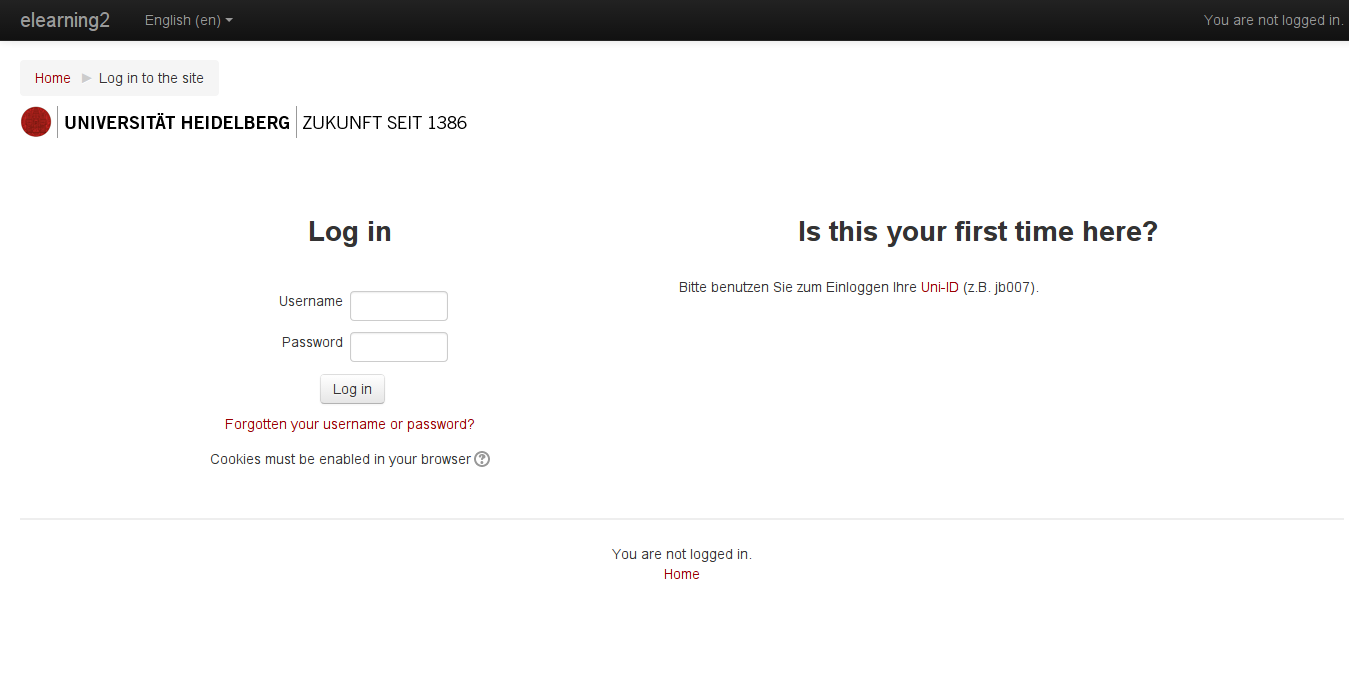
\includegraphics[width=\paperwidth]{moodle_anm_2014.png}}
\end{frame}
\begin{frame}{Startseite}
    \vspace*{10pt}
    \makebox[\linewidth]{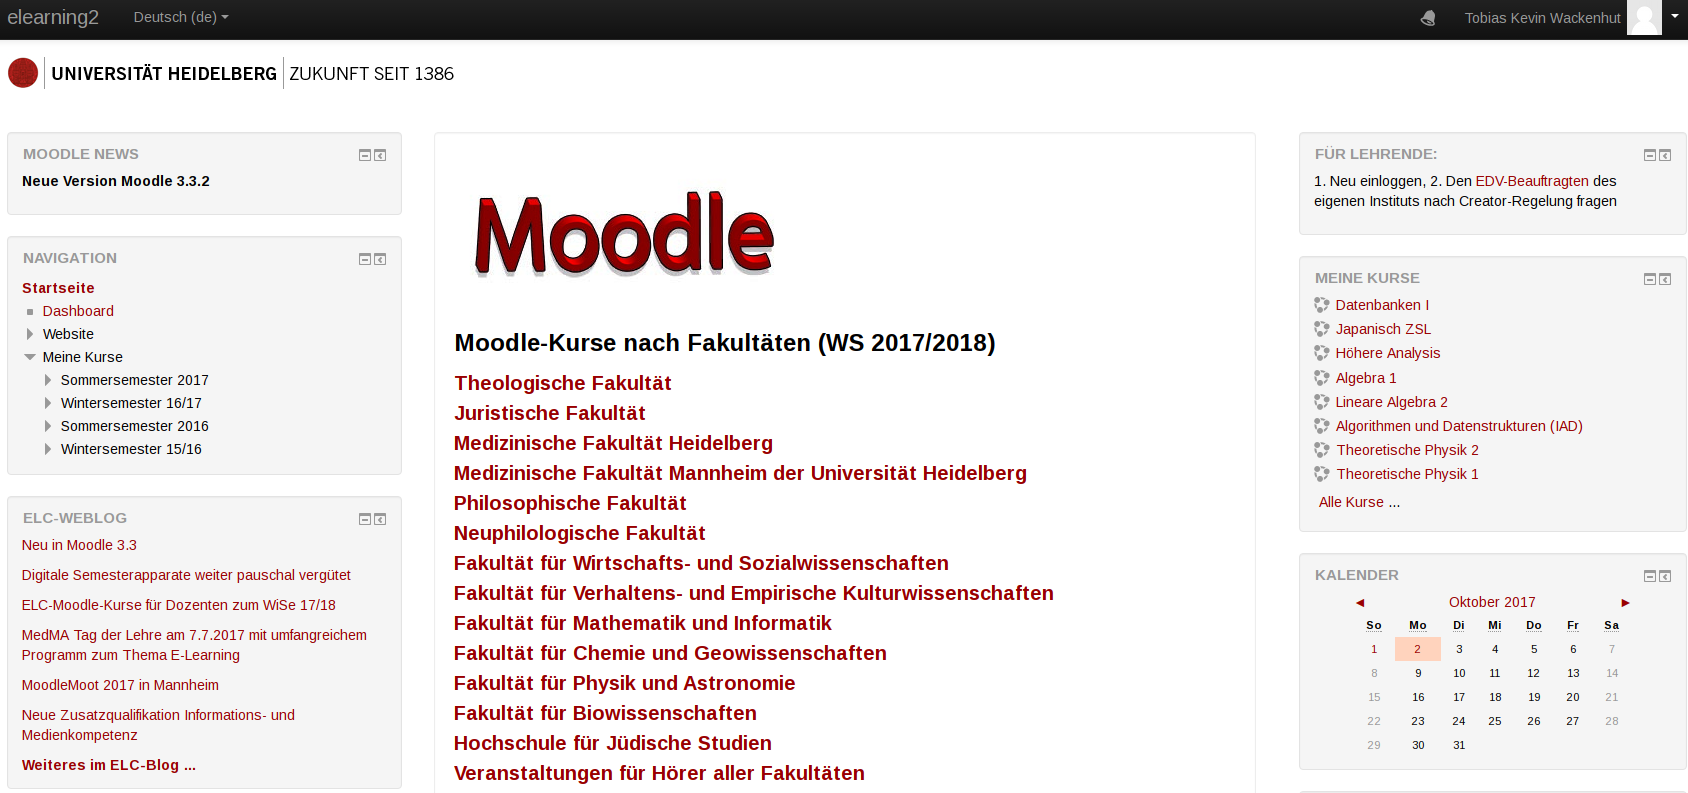
\includegraphics[width=\paperwidth]{moodle_startscreen.png}}
\end{frame}

\begin{frame}{Dashboard}
    \vspace*{10pt}
    \makebox[\linewidth]{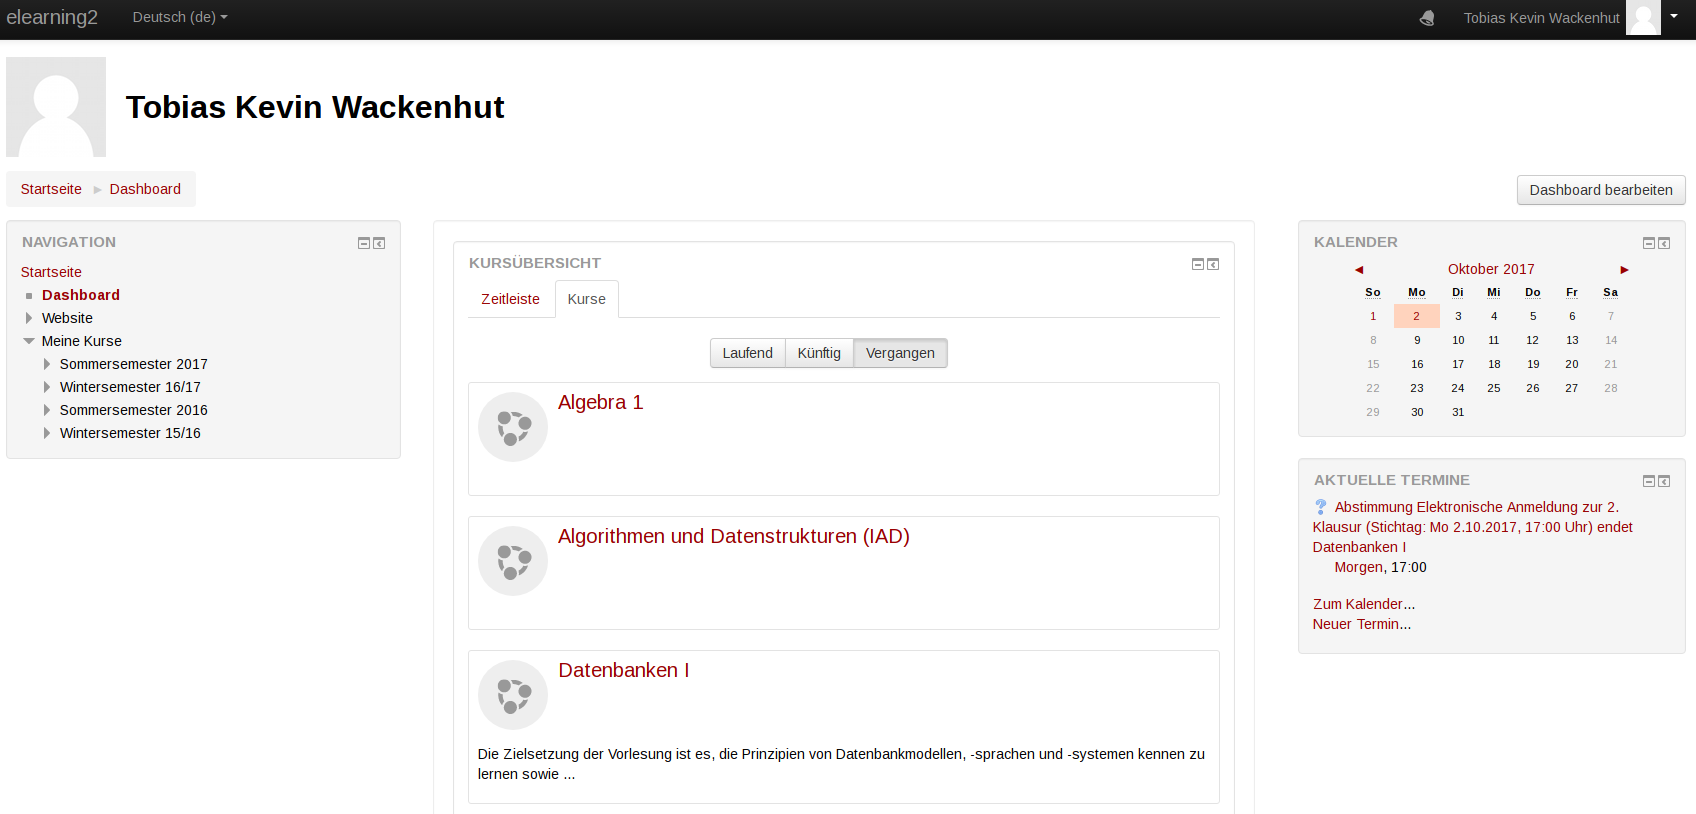
\includegraphics[width=\paperwidth]{moodle_dashboard.png}}
\end{frame}

\begin{frame}{Vorlesungen}
    \vspace*{10pt}
    \makebox[\linewidth]{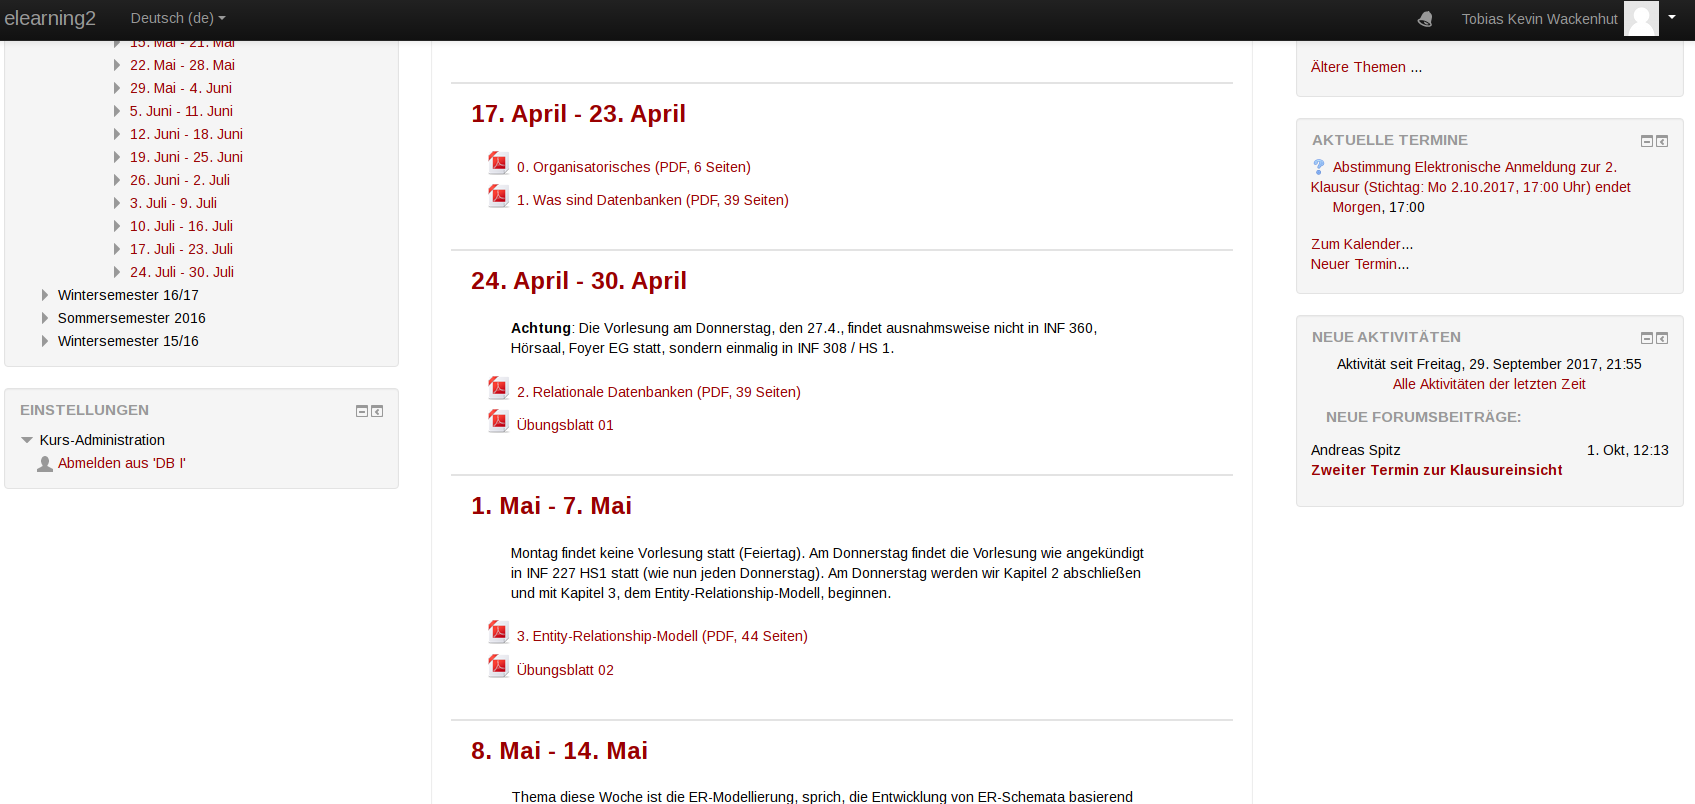
\includegraphics[width=\paperwidth]{moodle_vorlesungen.png}}
\end{frame}

\begin{frame}{Und wo finde ich das jetzt?}
    \begin{center}
        \huge{\textbf{Google}:}\\
        \vspace{1em}
        \huge{\frqq moodle uni hd\flqq}\\
        \vspace{2em}
        \visible<2>{
			\huge{\href{https://elearning2.uni-heidelberg.de}{elearning2.uni-heidelberg.de}}
        }
    \end{center}
\end{frame}

\section{Das LSF}
\begin{frame}{Das LSF}
        \vspace*{10pt}
    \makebox[\linewidth]{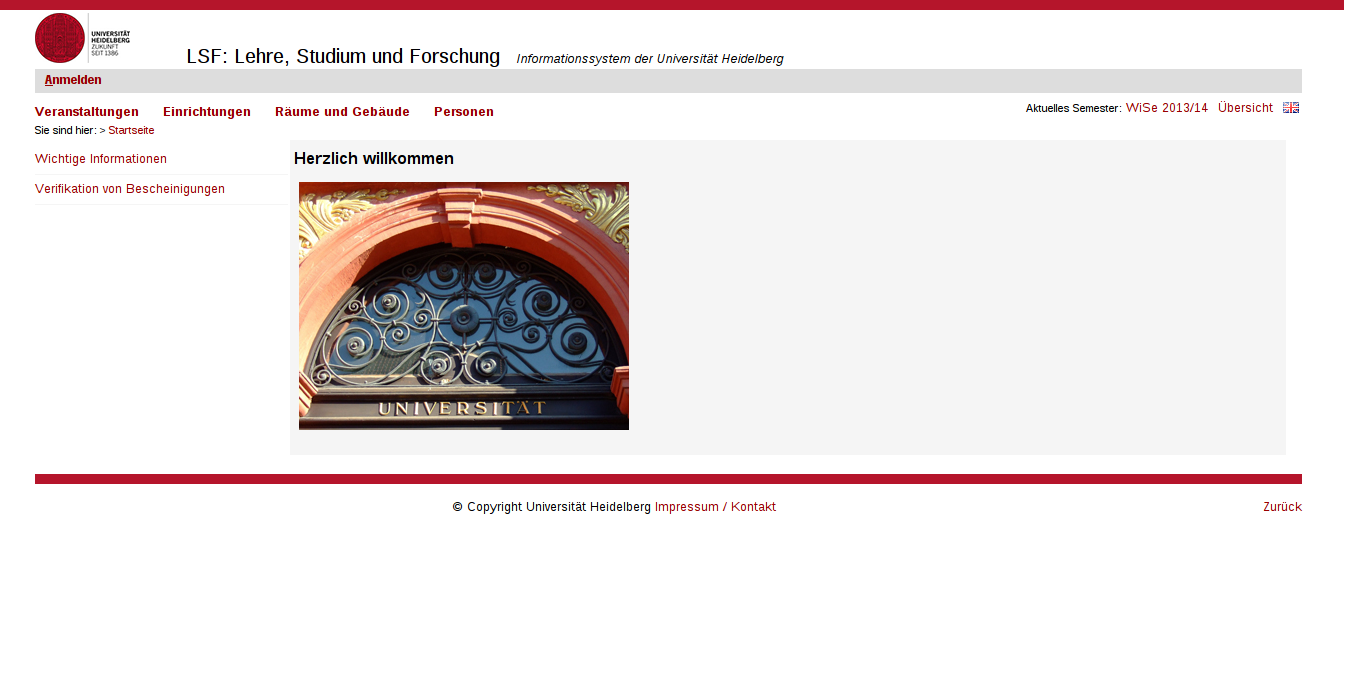
\includegraphics[width=\paperwidth]{LSF_start}}
\end{frame}

\begin{frame}{Anmeldung beim LSF}
        \vspace*{-5pt}
    \makebox[\linewidth]{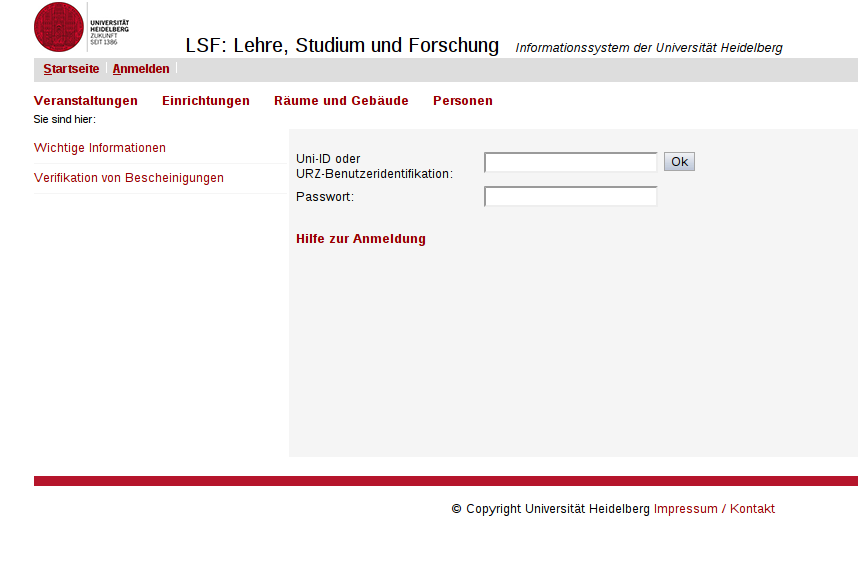
\includegraphics[width=\paperwidth]{LSF_anm}}
\end{frame}

\begin{frame}{Studiumsverwaltung}
        \vspace*{-5pt}
    \makebox[\linewidth]{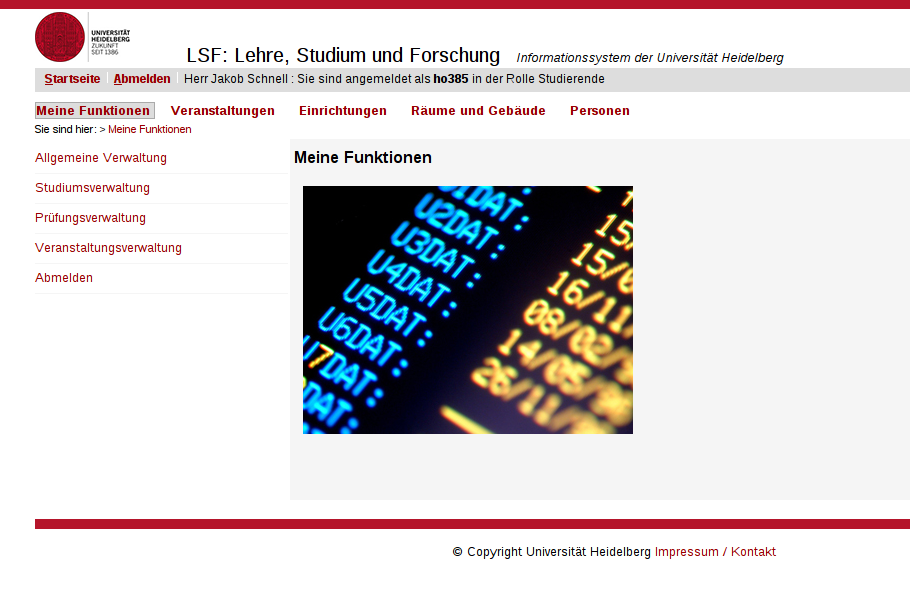
\includegraphics[width=\paperwidth]{LSF_funkt}}
\end{frame}

\begin{frame}{Vorlesungsverzeichnis Übersicht}
        \vspace*{-5pt}
    \makebox[\linewidth]{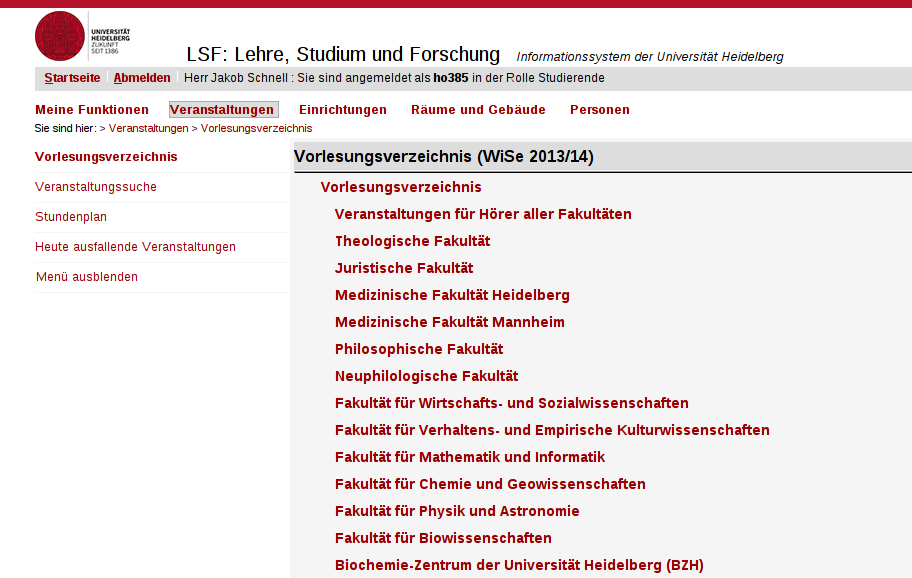
\includegraphics[width=\paperwidth]{LSF_VVZ_fak}}
\end{frame}

\begin{frame}{Vorlesungsverzeichnis Fakultätsebene}
        \vspace*{-10pt}
    \makebox[\linewidth]{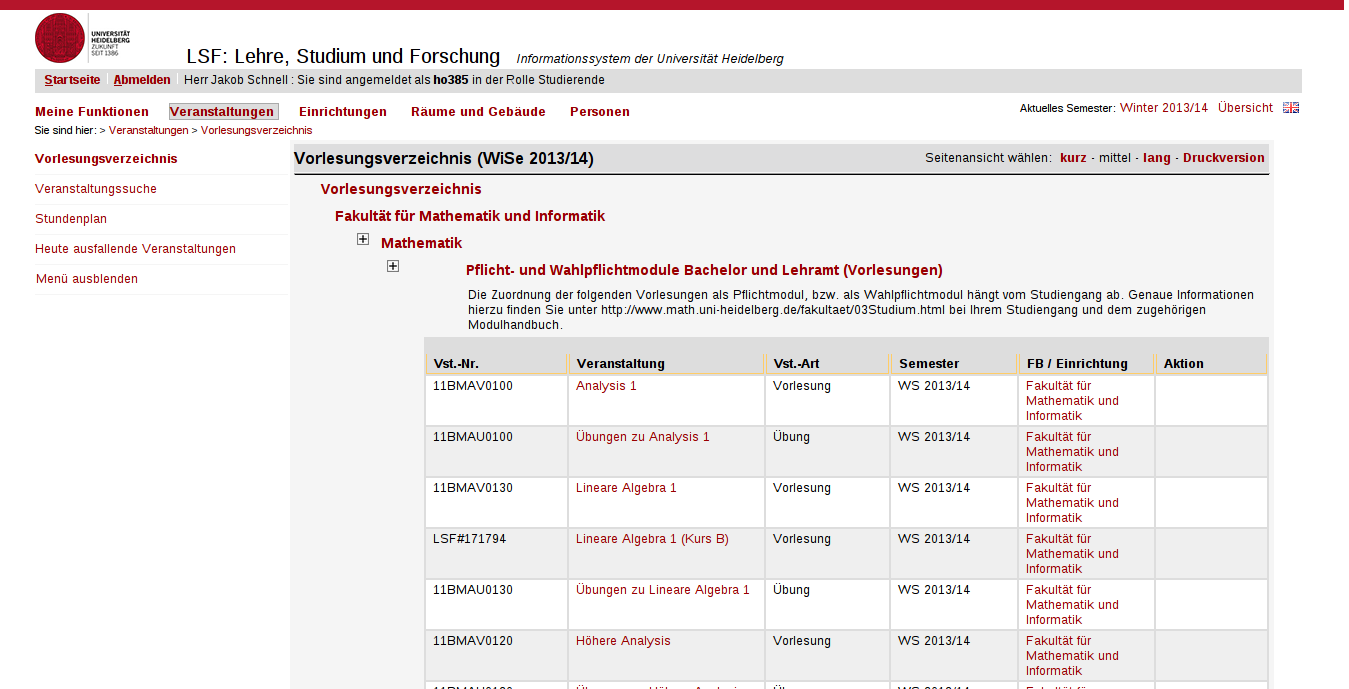
\includegraphics[width=\paperwidth]{LSF_VVZ_ueb}}
\end{frame}

\begin{frame}{Vorlesungsverzeichnis Veranstaltung}
		\vspace*{-5pt}
	\makebox[\linewidth]{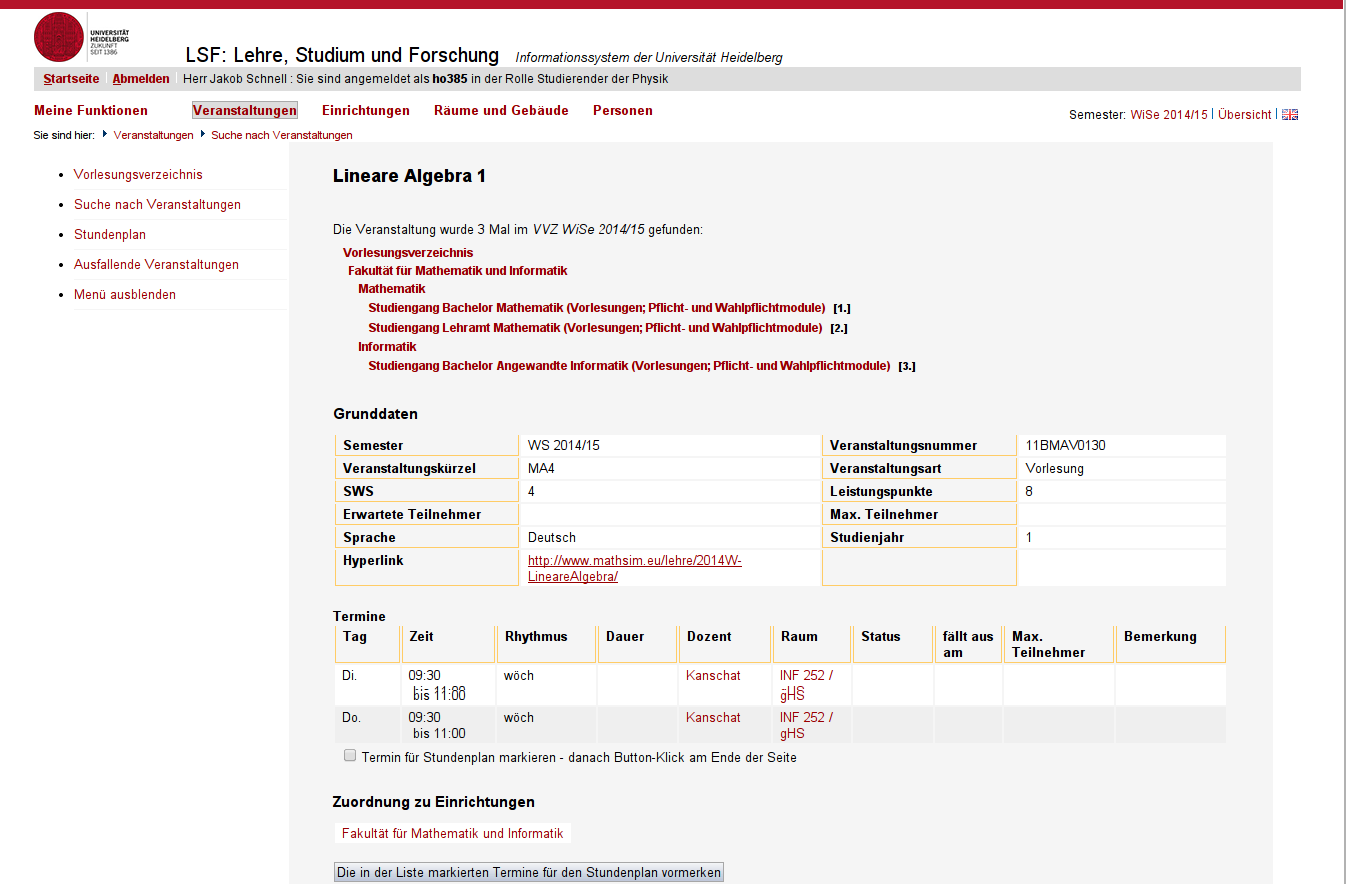
\includegraphics[width=\paperwidth]{LSF_VL}}
\end{frame}

\begin{frame}{Und wo finde ich das jetzt?}
    \begin{center}
        \huge{\textbf{Google}:}\\
        \vspace{1em}
        \huge{\frqq lsf uni hd\flqq}\\
        \vspace{2em}
        \visible<2>{
			\huge{\href{https://lsf.uni-heidelberg.de}{lsf.uni-heidelberg.de}}
        }
    \end{center}
\end{frame}

\section{Das Müsli}
\begin{frame}{Das Müsli}
        \vspace*{-50pt}
    \makebox[\linewidth]{
\includegraphics[width=\paperwidth]{muesli_start}}
\end{frame}

\begin{frame}{Registrieren beim Müsli}
        \vspace*{-10pt}
    \makebox[\linewidth]{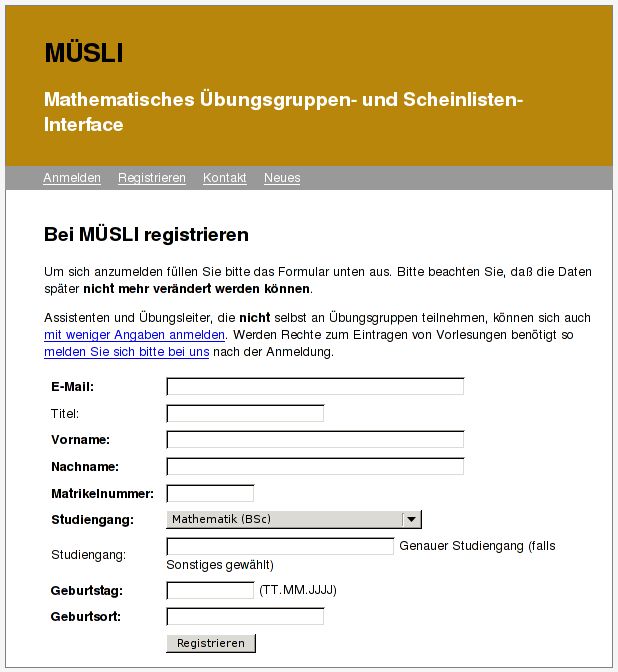
\includegraphics[width=\paperwidth]{muesli_anm}}
\end{frame}

\begin{frame}{Vorlesungsübersicht im Müsli}
        \vspace*{-50pt}
    \makebox[\linewidth]{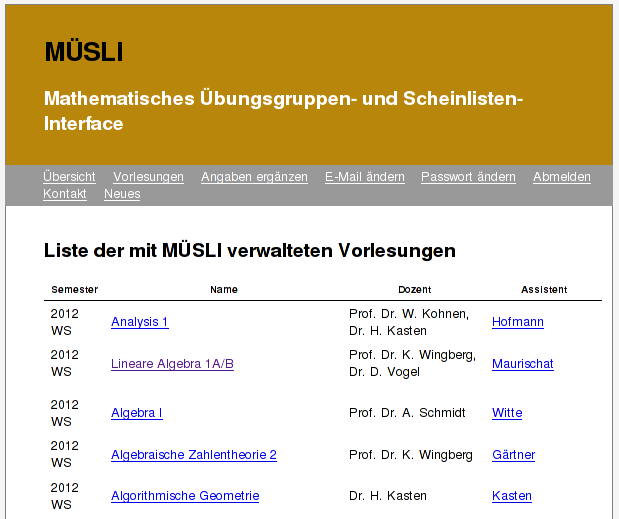
\includegraphics[width=\paperwidth]{muesli_vorl}}
\end{frame}

\begin{frame}{Übungsgruppenanmeldung im Müsli}
        \vspace*{-50pt}
    \makebox[\linewidth]{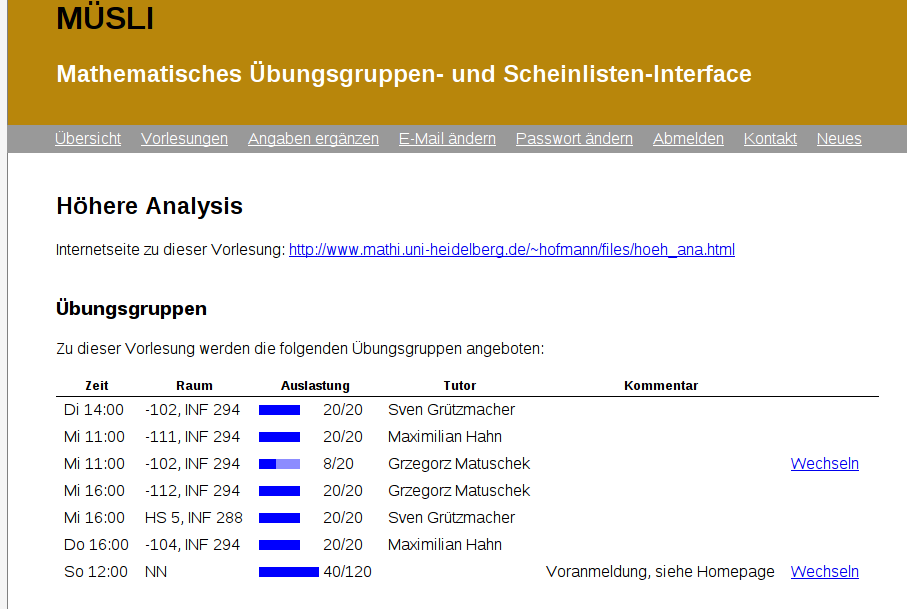
\includegraphics[width=\paperwidth]{muesli_ueb}}
\end{frame}

\begin{frame}{Startseite im Müsli}
        \vspace*{-40pt}
    \makebox[\linewidth]{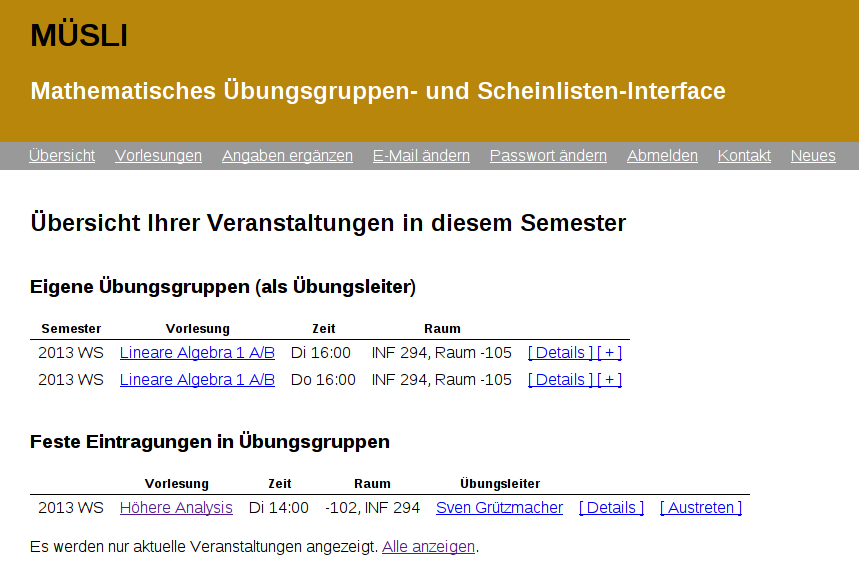
\includegraphics[width=\paperwidth]{muesli_home}}
\end{frame}

\begin{frame}{Punkteübersicht im Müsli}
        \vspace*{-40pt}
    \makebox[\linewidth]{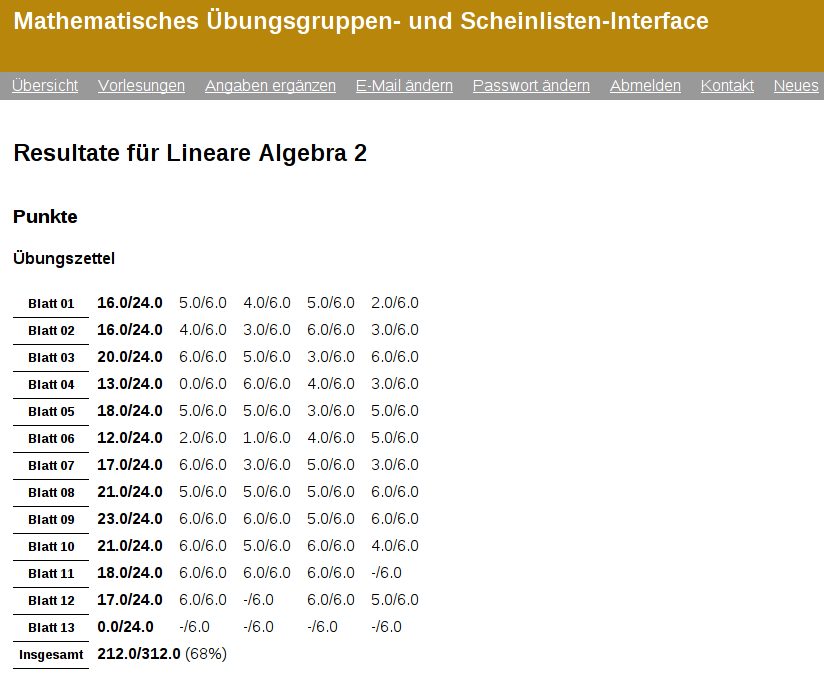
\includegraphics[width=\paperwidth]{muesli_pkte}}
\end{frame}

\begin{frame}{Und wo finde ich das jetzt?}
    \begin{center}
        \huge{\textbf{Google}:}\\
        \vspace{1em}
        \huge{\frqq müsli uni hd\flqq}\\
        \vspace{2em}
        \visible<2>{
			\huge{\href{https://muesli.mathi.uni-heidelberg.de/}{muesli.mathi.uni-heidelberg.de}}
        }
    \end{center}
\end{frame}

\begin{frame}{Fragen}
    \begin{center}
        \vfill
        \huge{\textbf{Was sind eure Fragen?}}\\
        \vfill
    \end{center}
\end{frame}

\begin{frame}{Und jetzt?}
    \begin{center}
            \huge{\textbf{Training}}:\\
            \vspace{1em}
			\huge{Übungsgruppen-Anmeldung}\\
			\pause\huge{\href{https://mathphys.fsk.uni-heidelberg.de/vorkurs/workshops}{Workshop-Anmeldung}}
    \end{center}
\end{frame}

\begin{frame}{MaMpf}
    \begin{center}
        \vfill
        \huge{\textbf{MaMpf}}\\\normalsize
	\begin{itemize}
		\item In Entwicklung
		\item verschiedene Teilprojekte
		\item[]
		\item \href{https://mampf.mathi.uni-heidelberg.de/}{mampf.mathi.uni-heidelberg.de}
	\end{itemize}
        \vfill
    \end{center}
\end{frame}
\end{document}
